\chapter{Tutorial}

This tutorial is tested since MATSim 0.4.0. This version is written for use with MATSim 0.7.0, but is still under construction. 

\section{Introduction}

The MATSim contrib for traffic lights is able to simulate traffic signals microscopically. 
For fixed-time control a default implementation is provided.  
No programming is required to simulate fixed-time traffic signal control. 
Traffic-responsive signal control needs custom implementation but can benefit from the provided infrastructure. 



\subsection{Terminology}

To help you to understand xml formats, configuration, and code better, have a look at the terminology in Fig.~\ref{fig:signals_terminology}. 

\begin{figure}[!h]
	\centering
\begin{tabularx}{\linewidth}{p{0.2\linewidth}p{0.3\linewidth}X}
	\textbf{MATSim term} & \textbf{Real world terms} & \textbf{Description} \\ 
& &  \\
signal & traffic light, traffic signal & A physical box standing somewhere on the transport network indicating driving allowed/permitted \\ 
signal group & a group of traffic lights & Logical group of traffic lights, all lights display same color at the same time \\ 
signal control & traffic controller & Algorithm or control scheme that determines which colors are displayed by the different Signal Groups, e.g. fixed-time control  \\ 
signal system & signalized crossing &  Collection of Signal Groups that is controlled by the same Signal Control 
\end{tabularx}
	\caption{Terminology}
	\label{fig:signals_terminology}
\end{figure}

\subsection{Overview}

The contrib consists of several modules. None of them is required if you are willing to code yourself. 
The codebase is written under the assumption that the following features are optional:   

\begin{itemize}
	\item Lanes
	\item Intergreens
\end{itemize}

Both are required under certain circumstances, only. 
See the upcoming MATSim book for further hints. 

\subsubsection{Lanes}

TBD.

\subsubsection{Intergreens}

MATSim's queue model implementation does not contain any collision detection. 
That is, a signal control can switch several conflicting approaches to green at the same time. 
The simulation does not report any error. 

To prevent such faulty behavior, the intergreens component can be switched on. 
An xml file defines for each signal system the intergreen times of the signal groups, i.e. the minimal time period between the ending of the one and the beginning of the other signal groups green phase. 
This information is then used to validate the signal control while the simulation is executed and may result in a warning or an exception. 

This is especially important if you implement a custom, traffic-responsive signal control strategy.  


\section{Usage \& Configuration}
\label{sec:signals_configuration}

\subsection{Usage}

\begin{itemize}
	\item Include the .jar file of the contrib into your java classpath
	\item Write a java \lstinline$main(..)$ method that loads your config and contains the following lines of code:
		\begin{lstlisting}
Scenario scenario = ScenarioUtils.loadScenario( config ) ;
SignalSystemsConfigGroup signalsConfigGroup = ConfigUtils.addOrGetModule(config, 
		SignalSystemsConfigGroup.GROUPNAME, SignalSystemsConfigGroup.class);
scenario.addScenarioElement(SignalsData.ELEMENT_NAME, 
		new SignalsScenarioLoader(signalsConfigGroup).loadSignalsData());

Controler c = new Controler( scenario );
c.addOverridingModule(new SignalsModule());
		\end{lstlisting}
	\item Execute \lstinline$c.run(..)$ somewhere in your \lstinline$main(..)$
\end{itemize}



\subsection{Config Options}

If input files for signal systems are already available, simulation of traffic lights can be enabled via MATSim config options:

\begin{itemize}
	\item Set at least three input file names in the config module signalsystems:
		\begin{itemize}
			\item parameter name: \lstinline$useSignalsystems$ value: \lstinline$true$ or \lstinline$false$
			\item parameter name: \lstinline$signalsystems$ value: path to a file in the \lstinline$signalSystems_v2.0.xsd$ file format
  		\item parameter name: \lstinline$signalgroups$ value: path to a file in the \lstinline$signalGroups_v2.0.xsd$ file format
 			\item parameter name: \lstinline$signalcontrol$ value: path to a file in the \lstinline$signalControl_v2.0.xsd$ file format
 			\item parameter name: \lstinline$useAmbertimes$ (optional) value: \lstinline$true$ or \lstinline$false$
 			\item parameter name: \lstinline$ambertimes$ (optional) value: path to a file in the \lstinline$amberTimes_v1.0.xsd$ file format
			\item parameter name: \lstinline$useIntergreenTimes$ (optional) value: \lstinline$true$ or \lstinline$false$
			\item parameter name: \lstinline$intergreentimes$ (optional) value: path to a file in the \lstinline$intergreenTimes_v1.0.xsd$ file format
			\item parameter name: \lstinline$actionOnIntergreenViolation$ (optional) value: \lstinline$warn$ or \lstinline$exception$
		\end{itemize}
\end{itemize}




\section{Further Reading}

A conceptual introduction to this MATSim contribution can be found in \cite{Grether2014PhD}. 
For case studies in German, see \cite{Bischoff2010BaSylvia,Neumann2008DA,Roeder2010BachelorGershenson}.

\section{Generating Input Data -- Example}

There is a small example in order to help you getting started, the class is RunCreateTrafficSignalScenarioExample.

The example uses the network shown in Figure~\ref{fig:RunCreateTrafficSignalScenarioExampleNetwork}. 

\begin{figure}[htbp]
	\center
	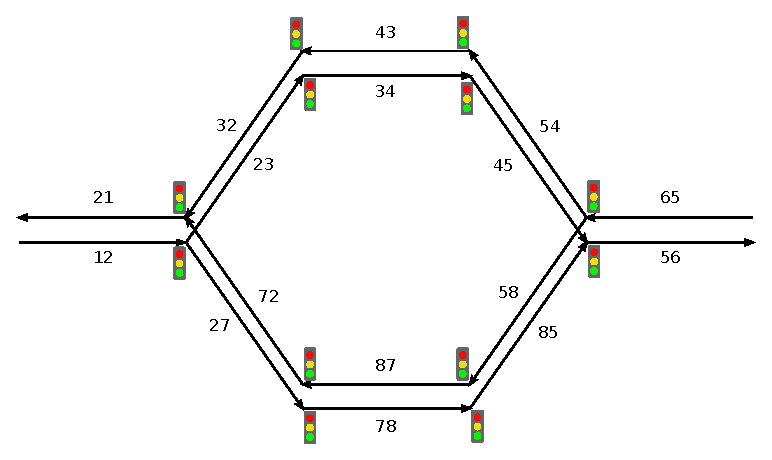
\includegraphics{data/RunCreateTrafficSignalScenarioExampleNetwork}
	\caption{Network used by the scenario in RunCreateTrafficSignalScenarioExample. The numbers show the link ids. Traffic lights to be created are shown as small icons.}
	\label{fig:RunCreateTrafficSignalScenarioExampleNetwork}
\end{figure}

The following highlights important lines of code method by method.

\subsubsection{Code}

Input files for the examples can be found in the folder  contribs/signals/examples/tutorial/example90TrafficLights of the current MATSim release.

Example code can be found in the folder src/main/java in the package tutorial.trafficsignals in the signals contrib.

\subsubsection{RunCreateTrafficSignalScenarioExample.run()}

This method sets up the config and writes the signals that are created in submethods to file.

As optional module, the signal systems module has to be switched on in the scenario first:


\texttt{\nolinebreak config.setUseSignalSystems(true);}

Then, qsim as mobility simulation should be used:


\texttt{\nolinebreak config.controler().setMobsim("qsim"); \nolinebreak }


After the scenario is loaded, the top-level container for all signal related data has to be added: 


\texttt{\nolinebreak SignalSystemsConfigGroup signalsConfigGroup = ConfigUtils.addOrGetModule(config, SignalSystemsConfigGroup.GROUPNAME, SignalSystemsConfigGroup.class);}

\texttt{\nolinebreak scenario.addScenarioElement(SignalsData.ELEMENT\_NAME, new SignalsScenarioLoader(signalsConfigGroup).loadSignalsData());}

and is afterwards retrieved by: 

\texttt{\nolinebreak SignalsData signalsData = (SignalsData) scenario.getScenarioElement(SignalsData.ELEMENT\_NAME);}

\subsubsection{RunCreateTrafficSignalScenarioExample.createSignalSystemsAndGroups(..)}

This method creates the physics, i.e. locations of signals. Furthermore SignalGroups for the Signals are created.

First a SignalSystem has to be created and explicitly added to the container:


\texttt{\nolinebreak SignalSystemData sys = systems.getFactory().createSignalSystemData(Id.create("3", SignalSystem.class));
\\  \nolinebreak systems.addSignalSystemData(sys);}

Then on link 23 a Signal with Id 1 can be created:


\texttt{\nolinebreak SignalData signal = systems.getFactory().createSignalData(Id.create("1", Signal.class));
\\\nolinebreak sys.addSignalData(signal);
\\\nolinebreak signal.setLinkId(Id.create("23", Link.class));}

The Signal must be added to the SignalSystem after creation.

This is continued until all Signals of the SignalSystem are created.

We then need some SignalGroup for the Signals. In this example each Signal has its\nolinebreak own group. That is done by calling:


\texttt{\nolinebreak SignalUtils.createAndAddSignalGroups4Signals(groups, sys);}

\subsubsection{RunCreateTrafficSignalScenarioExample.createSignalControl(..)}

This method adds a fixed-time traffic signal control on top of the SignalGroups created by the last method. The SignalGroups control the hardware, i.e. the Signals. MATSim Events are created for SignalGroups.

Each SignalSystem is equiped with a fixed-time control. Each SignalSystem is setup the same way: A cycle time of 120 sec is used. Each direction gets green for second 0 to 55 within the cycle. Offsets for green waves are set to 0 seconds.

The Code can be read as follows:

Create a fixed-time control and add it to the container:


\texttt{\nolinebreak  SignalSystemControllerData controller = control.getFactory().createSignalSystemControllerData(id); \\ \nolinebreak control.addSignalSystemControllerData(controller); \\ \nolinebreak controller.setControllerIdentifier( DefaultPlanbasedSignalSystemController.IDENTIFIER);\nolinebreak }

Then, create a fixed-time control plan (a plan can be disabled or changed at a certain time of day) and add it to the container:


\texttt{\nolinebreak    SignalPlanData plan = control.getFactory().createSignalPlanData(Id.create("1", SignalPlan.class));\\ \nolinebreak    controller.addSignalPlanData(plan);\nolinebreak  }

Each fixed-time control plan has specific attributes for cycle and synchronization offset:


\texttt{\nolinebreak    plan.setCycleTime(cycle);\\ \nolinebreak   plan.setOffset(0);\nolinebreak }

Create specific green times (onset = switch to green, offset = switch to amber/red) for all SignalGroups and add them to the signal control plan via


\texttt{\nolinebreak    SignalGroupSettingsData settings1 = control.getFactory().createSignalGroupSettingsData(Id.create("1", SignalGroup.class));\\ \nolinebreak   plan.addSignalGroupSettings(settings1);\\ \nolinebreak   settings1.setOnset(0);\\ \nolinebreak   settings1.setDropping(55);\\ \nolinebreak }

\subsubsection{Visualization}

If you want to visualize the created scenario try to get and run the OTFVis contribution to MATSim (use MATSim head or nightly build instead of 0.4.1), see \href{http://matsim.org/docs/extensions/otfvis}{OTFVis}(this contribution is unsupported, please submit patches instead of mails).

If OTFVis runs successfully, you may be able to run


\texttt{\nolinebreak  tutorial.trafficsignals.VisSimpleTrafficSignalScenario }

within an up to date (> 04.12.2012) checkout within eclipse.

Another option is to write the scenario to file via the example code and then start OTFVis with the created config file.

\subsection{Links}
\begin{itemize}
	\item \href{http://ci.matsim.org:8080/job/MATSim_M2/javadoc/org/matsim/signalsystems/package-summary.html}{Technical Documentation (JavaDoc)}
	\item \href{http://matsim.org/node/693}{OTFVis}
	\item \href{https://opus4.kobv.de/opus4-tuberlin/frontdoor/index/index/docId/5325}{Dissertation of D. Grether}	
\end{itemize}

\subsection{Intergreens}

There is a small example how to create an intergreen xml file with given
intergreen times for specific signal groups (see
tutorial.trafficsignals.RunCreateIntergreensExample.java).

If there is no intergreen data available for your scenario you may use the
intergreen times of a correct fixed time signal control, i.~e. a signal control
with realistic intergreen times where no collisions may occur (therefor you may
look at playground.dgrether.signalsystems.sylvia.data.TtCalculateSimplifiedIntergreens.java).

\section{Input Files -- Examples}

\subsection{Intergreens}
\lstset{breaklines=true,language=XML}
\lstinputlisting{../../src/test/resources/test/input/org/matsim/contrib/signals/data/intergreens/v10/testIntergreenTimes_v1.0.xml}


\texttt{\nolinebreak  }




\texttt{\nolinebreak  }
